\documentclass[14pt]{extreport}
\usepackage[utf8]{vietnam}
%\usepackage{type1cm}
\usepackage[left=3.50cm, right=2.00cm, top=3.50cm, bottom=3.00cm]{geometry}
%\usepackage[left=3.0cm, right=1.50cm, top=3.00cm, bottom=2.50cm]{geometry}
\usepackage{graphicx}
\usepackage{mathrsfs} 
\usepackage{amsfonts}
\usepackage{longtable}
\usepackage[intlimits]{amsmath}
\usepackage{array}
\usepackage{amsxtra,amssymb,latexsym,amscd,amsthm}
\usepackage{algorithm}
\usepackage{algorithmic}
\newtheorem{theorem}{\MakeUppercase{K}ết quả}[section]
% khoảng cách dòng 1.5 lines (như trong MS Word)
\renewcommand{\baselinestretch}{1.5}

%——————–
\begin{document}
%tao khung
\newcommand{\Khung}[2]{
\begin{tabular}{|l|}
\hline\rule[-2ex]{0pt}{5.5ex}
\parbox{#1}{#2}\\
\hline
\end{tabular}
}

\Khung{.92\textwidth}{

\begin{center}
\normalsize
\textbf{TRƯỜNG ĐẠI HỌC BÁCH KHOA HÀ NỘI}\\
\normalsize
\textbf{VIỆN TOÁN ỨNG DỤNG VÀ TIN HỌC}\\
\textbf{------------------------------------------------------}\\[0.4cm]

\includegraphics[scale=.2]{logobkdentrang}\\[1.2cm]
\textbf{{\large NGÔN NGỮ CHÍNH QUY, BIỂU THỨC CHÍNH QUY VÀ SƠ LƯỢC VỀ LÝ THUYẾT MÃ}}\\
\end{center}
\begin{flushleft}
\vspace{1.3cm}
\hspace{1.5cm} \textbf{ Giáng viên hướng dẫn:{ TS. Ngô Thị Hiền }}\\[0.2cm]
\hspace{1.5cm} \textbf{ Nhóm Sinh viên thực hiện:}\\[0.2cm]
\hspace{5cm}\textbf{Nguyễn Anh Tú}\\[0.2cm]
\hspace{5cm}\textbf{Phạm Anh Tuấn}\\[0.2cm]
\hspace{1.5cm} \textbf{ Lớp:\hspace{2cm}{ KSTN Toán Tin K60}}\\
\end{flushleft}

\begin{center}
\textbf{{\small HÀ NỘI - 12/2018}}\\
\end{center}
 }
\thispagestyle{empty}
\newpage

\tableofcontents
\newpage

%\listoffigures

\newpage

\chapter{Giới thiệu}
Ngôn ngữ là phương tiện để giao tiếp, sự giao tiếp có thể hiểu là giao tiếp giữa con người với nhau, giao tiếp giữa người với máy, hay giao tiếp giữa máy với máy. Ngôn ngữ để con người có thể giao tiếp với nhau được gọi là ngôn ngữ tự nhiên, chẳng hạn như tiếng Anh, tiếng Việt… là các ngôn ngữ tự nhiên. Các quy tắc cú pháp của ngôn ngữ tự nhiên nói chung rất phức tạp nhưng các yêu cầu nghiêm ngặt về ngữ nghĩa thì lại thiếu chặt chẽ, chẳng hạn cùng một từ hay cùng một câu ta có thể hiểu chúng theo những nghĩa khác nhau tùy theo từng ngữ cảnh cụ thể. Con người muốn giao tiếp với máy tính tất nhiên cũng thông qua ngôn ngữ. Để có sự giao tiếp giữa người với máy hay giữa máy với nhau, cần phải có một ngôn ngữ với các quy tắc cú pháp chặt chẽ hơn so với các ngôn ngữ tự nhiên, nói cách khác, với một từ hay một câu thì ngữ nghĩa của chúng phải là duy nhất mà không phụ thuộc vào ngữ cảnh. Những ngôn ngữ như thế được gọi là ngôn ngữ hình thức. Con người muốn máy tính thực hiện công việc, phải viết các yêu cầu đưa cho máy bằng ngôn ngữ máy hiểu được. Việc viết các yêu cầu như thế gọi là lập trình. Ngôn ngữ dùng để lập trình được gọi là ngôn ngữ lập trình. Các ngôn ngữ lập trình đều là các ngôn ngữ hình thức. 

Trong bài báo cáo này, nhóm em sẽ trình bày về ngôn ngữ chính quy, biểu thức chính quy và sơ lược về lý thuyết mã. Ngôn ngữ chính quy (regular languages) thường được biết đên nhờ ứng dụng trong việc tìm từ trong văn bản hay trong trình dịch. Tuy nhiên, trong khuôn khổ của bài báo cáo này, nhóm chúng em sẽ tập trung trình bày những tính chất của ngôn ngữ chính quy và đi giải quyết các bài toán liên quan đến việc biểu diễn và cực tiểu hóa các cách biểu diễn của ngôn ngữ chính quy. Về nội dung của phần lý thuyết mã, bài báo cáo sẽ trình bày những kết quả cơ bản trong lý thuyết mã và một ứng dụng quan được sử dụng rỗng rãi trong trong việc truyền thông tin đó là mã sửa sai.


\chapter{Kiến thức cơ sở}
\section{Xâu}
Bảng chữ cái là một tập hợp các kí tự (có thể gồm hữu hạn hoặc vô hạn các phần tử). Xâu là một dãy hữu hạn các kí tự thuộc bảng chữ cái. Độ dài của xâu là số các kí tự trong xâu đó. Xấu rỗng, được kí hiệu là $\epsilon$, độ dài xâu rồng bằng 0.\\
Xâu $s$ được gọi là xâu con của $w$ nếu $\exists s_0, s_1$ sao cho $s_0ss_1 = w$. Đặc biệt:
\begin{itemize}
\item Nếu $s_0 =\epsilon$ thì $s$ được gọi là prefix của $s$
\item Nếu $s_1 =\epsilon$ thì $s$ được gọi là suffix của $s$
\end{itemize}

\textbf{Các phép toán trên xâu}
\begin{enumerate}
\item Tích ghép
Cho 2 xâu: $a=a_1a_2...a_n,b=b_1b_2...b_m$ trên bảng chữ cái $A$. Tích ghép của hai xâu $a$, $b$ là xâu $c=ab=a_11_2...a_nb_1b_2...b_m$

Nhận xét: Cho các xâu $s,r,w$ trên bảng chữ cái $A$
\begin{itemize}
\item Xâu rỗng là phần tử đơn vị với phép nối xâu

$s\epsilon =\epsilon s=s$
\item Phép ghép nối có tính chất kết hợp

$\left(sr\right)w=s\left(rw\right)$
\item Kí hiệu $w^n$, với $n$ là số tự nhiên

$w^n=\left\{\begin{matrix}
\epsilon ,n=0\\ 
w,n=1\\ 
w^{n-1}w, n>1
\end{matrix}\right.$
\end{itemize}
\item Phép đảo ngược xâu

$w^R$ được gọi là xâu đảo ngược của $w$ nếu:

$w^{R}=\left\{\begin{matrix}
\epsilon, w=\epsilon \\ 
s_ns_{n-1}...s_0, w=s_0...s_{n-1}s_n; s_i \in A,i=\overline{1,n}
\end{matrix}\right.$

Cho xâu $s,w$. Phép đảo ngược xâu có các tính chất sau:
\begin{itemize}
\item ${\left(w^R\right)}^R=w$
\item ${\left(sw\right)}^R=w^Rs^R$
\item $\left|w^R\right|=\left|w\right|$
\end{itemize}
\end{enumerate}

\section{Ngôn ngữ}
Ngôn ngữ là tập các xâu trên một bảng chữ cái.\\
\textbf{Các phép toán trên ngôn ngữ} \\
Xét hai ngôn ngữ $L_1,L_2$ trên bảng chữ cái $A$
\begin{enumerate}
\item Phép tích ghép

Cho ngôn ngữ $L_1$ trên bảng chữ cái $A_1$, $L_2$ trên bảng chữ cái $A_2$. Phép nhân ghép của hai ngôn ngữ $L_1,L_2$ là một ngôn ngữ trên bảng chữ cái $A_1 \cup A_2$, kí hiệu $L_1L_2$:
\begin{center}
$L_1L_2=\left\{ab|a\in L_1,b\in L_2\right\}$
\end{center}

Nhận xét: Xét các ngôn ngữ $L_1,L_2,L_3$.Phép nhân ghép có các tính chất sau
\begin{itemize}
\item Tính chất kết hợp: $\left(L_1 L_2 \right) L_3=L_1 \left(L_2 L_3 \right)$
\item $\forall L_1:L_1 \varnothing =\varnothing L_1=\varnothing$
\item Tính chất phân phối đối với phép nhân ghép và phép hợp:
\begin{center}
$\left(L_1\cup L_2\right) L_3=\left(L_1 L_3 \right)\cup \left(L_2  L_3\right)$

$L_1\left( L_2\cup L_3\right)=\left(L_1 L_3 \right)\cup \left(L_2 L_3\right)$

\end{center}
\end{itemize}

\item Phép toán sao

Ta định nghĩa $L^n$ là phép tích ghép của $n$ lần ngôn ngữ $L$
$$L^n = \prod_{i=0}^n L$$
Trong đó $L^0 = \epsilon$.Khi đó, phép toán sao trên ngôn ngữ $L$ được định nghĩa như sau
$$L^* = \bigcup_{i=0}^{\infty} L^i$$
Ta cũng định nghĩa
$$L^+ = L^* \setminus \{ \epsilon \}$$
Ở đây, ta có chú ý rằng $A*$ là một vị nhóm tự do đối với phép toán tích ghép.

\item Phép hợp

Hợp của hai ngôn ngữ $L_1,L_2$, kí hiệu $L_1\cup L_2$ là một ngôn ngữ trên bảng chữ cái $A$:

\begin{center}
$L_1\cup L_2=\{w\in A^*|w\in L_1$ hoặc $ w\in L_2\}$
\end{center}


Nhận xét: Xét các ngôn ngữ $L_1,L_2,L_3$.Phép hợp có các tính chất sau
\begin{itemize}
\item Tính chất giao hoán: $L_1\cup L_2=L_2\cup L_1$
\item Tính chất kết hợp: $\left(L_1\cup L_2 \right)\cup L_3=L_1\cup \left(L_2\cup L_3 \right)$
\item $\forall L1:L_1\cup \varnothing =\varnothing \cup L1=L1$ và $L_1 \cup A^*=A^*$
\end{itemize}

\item Phép giao

Giao của hai ngôn ngữ $L_1,L_2$, kí hiệu $L_1\cap L_2$
\begin{center}
$L_1\cap L_2=\{w\in A^*|w\in L_1$ và $ w\in L_2\}$
\end{center}

Nhận xét: Xét các ngôn ngữ $L_1,L_2,L_3$.Phép hợp có các tính chất sau
\begin{itemize}
\item Tính chất giao hoán: $L_1\cap L_2=L_2\cap L_1$
\item Tính chất kết hợp: $\left(L_1\cap L_2 \right)\cap L_3=L_1\cap \left(L_2\cap L_3 \right)$
\item $\forall L_1:L_1\cap \varnothing =\varnothing \cap L_1=\varnothing$ và $L_1 \cap A^*=L_1$
\item Tính chất phân phối đối với phép hợp và phép giao:
\begin{center}
$\left(L_1\cup L_2\right)\cap L_3=\left(L_1\cap L_3 \right)\cup \left(L_2 \cap L_3\right)$

$\left(L_1\cap L_2\right)\cup L_3=\left(L_1\cup L_3 \right)\cap \left(L_2 \cup L_3\right)$
\end{center}
\end{itemize}

\item Phép lấy phần bù
Ngôn ngữ phần bù của ngôn ngữ $L$ trên bảng chữ cái $A$, kí hiệu $C_AL$, là một ngôn ngữ trên bảng chữ cái $A$
\begin{center}
$C_AL=\{w\in A^*|w\notin L\}$
\end{center}

Nhận xét:Phép lấy phần bù có các tính chất sau
\begin{itemize}
\item $C_A\{\epsilon \}=A^+,C_AA^+=\{\epsilon \}$
\item $C_A \varnothing =A^*,C_AA^*=\varnothing$
\item $C_A\left(C_AL_1 \cup C_AL_2 \right)=L_1 \cap L_2$
\end{itemize}
\end{enumerate}

\section{Ngôn ngữ chính quy}
\subsection{Định nghĩa}

Ngôn ngữ chính quy được định nghĩa như sau:

\begin{enumerate}
\item $\varnothing$ là một ngôn ngữ chính quy
\item $\forall \in A,\left\{a\right\}$ là ngôn ngữ chính quy, $A$: bảng chữ cái
\item $L_1,L_2$ là các ngôn ngữ chính quy thì $L_1 \cup L_2,L_1L_2,L^*$ là các ngôn ngữ chính quy
\item Không có bất kì ngôn ngữ chính quy nào khác ngoài 1,2,3.
\end{enumerate}

\section{Biểu thức chính quy}
\subsection{Định nghĩa}

Một công cụ để biểu diễn ngôn ngữ chính quy là biểu thức chính quy. Biểu được định nghĩa như sau:

\begin{enumerate}
\item $\varnothing$ là biểu thức chính quy
\item $\epsilon$ là biểu thức chính quy
\item $a$ là ngôn ngữ chính quy với $a \in A$, $A$ là bảng chữ cái hữu hạn
\item $r,s$ là biểu thức chính quy

$\left\{\begin{matrix}
(r)(s)\rightarrow RS\\ 
r^{*}\rightarrow R^{*}
\\ (r)+(s)\rightarrow R\cup S

\end{matrix}\right.$ là các biểu thức chính quy
\end{enumerate}
\subsection{Các tính chất của biểu thức chính quy}

Cho $r,s,w$ là các biểu thức chính quy
\begin{enumerate}
\item $r+s=s+r$
\item $\left(r+s\right)+w=r+\left(s+w\right)$
\item $r\left(s+w\right)=rs+rw$
\item $r\epsilon=\epsilon r=r$
\item ${\left(\epsilon+r\right)}^*=r^*$
\item $r+\varnothing=r$
\item ${\left( r^*\right)}^*=r^*$
\item $r+r=r$
\item $r\left(sw\right)=\left(rs\right)w$
\item $\left(r+s\right)w=rw+sw$
\item $\varnothing r=r\varnothing=\varnothing$
\item $\varnothing^*=\epsilon$
\item $r+r^*=r^*$
\item ${\left(r^* s^*\right)}^*={\left(r+s\right)}^*$
\item ${\left(rs\right)}^*r=r{\left(sr\right)}^*$
\end{enumerate}
\subsection{Đồ thị biểu diễn biểu thức chính quy}
\begin{itemize}
\item Mỗi đỉnh là một vòng tròn, đỉnh kết thúc được biểu diễn là một vòng tròn nhân đôi
\item Đỉnh xuất phát thì mũi tên đi vào
\item Các toán tử được biểu diễn như sau:
\begin{center}
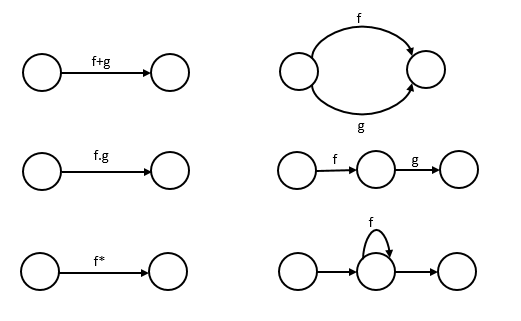
\includegraphics[scale=1.1]{dothibtcq}
\end{center}
\end{itemize}

\section{Automat hữu hạn}
\subsection{Automat đơn định(DFA)}
\begin{enumerate}
\item Quy luật để chuyển trạng thái mới cho bởi hàm chuyển:

$\delta: Q \times A\rightarrow Q$

$\delta(q,a)=p$

$q,p\in Q,a\in A$
\item Định nghĩa

$M$ là một DFA:
\begin{center}
$M=\left(A,Q,\delta,q_0,F\right)$
\end{center}
Trong đó:
\begin{itemize}
\item $A$: bảng chữ cái hữu hạn
\item $Q$: tập các trạng thái
\item $\delta$: hàm chuyển
\item $q_0$: trạng thái bắt đầu, $q_0 \in Q$
\item $F$: tập trạng thái kết thúc $F\subseteq Q$
\end{itemize}
\end{enumerate}

\subsection{Automat đa định(NFA)}
\begin{enumerate}
\item Quy luật để chuyển trạng thái mới cho bởi hàm chuyển:

$\delta: Q \times \left(A\cup \epsilon\right) \rightarrow 2^Q$

$\delta(q,a)=p$

$q\in Q, p \in 2^Q, a\in A$
\item Định nghĩa

$M$ là một DFA:
\begin{center}
$M=\left(A,Q,\delta,q_0,F\right)$
\end{center}
Trong đó:
\begin{itemize}
\item $A$: bảng chữ cái hữu hạn
\item $Q$: tập các trạng thái
\item $\delta$: hàm chuyển
\item $q_0$: trạng thái bắt đầu, $q_0 \in Q$
\item $F$: tập trạng thái kết thúc $F\subseteq Q$
\end{itemize}
\end{enumerate}
Mặc dù trong nhiều trường hợp, ta thấy rằng xây dựng NFA để đoán nhận một ngôn ngữ thường dễ hơn là xây dựng một NFA. Tuy nhiên, người ta đã chứng minh được rằng mọi ngôn ngữ được biểu diễn bởi một NFA nào đó đều có thể biểu diễn được bằng một DFA. Tuy nhiên, trong trượng hợp xấu nhất thì số lượng trạng thái của DFA là $2^n$ trong khi số lượng trạng thái của NFA là $n$. \\
\textbf{Định lý về sự tương đương.} Một ngôn ngữ $L$ được đoán nhận bởi một DFA nào đó khi và chỉ khi nó cũng được đoán nhận bởi một NFA nào đó
\section{Văn phạm}
\subsection{Định nghĩa}
Văn phạm $G$ là một bộ gồm 4 thành phần:
$$G = \{ V_T, V_N, S, P \}$$
trong đó:\\
\begin{enumerate}
\item $V_T$ là tập các kí tự kết thúc, mỗi kí tự của nó được gọi là một ký hiệu kết thúc.
\item $V_N$ là tập các kí tự không kết thúc, mỗi phần tử của nó được gọi là một ký hiệu không kết thúc hay ký hiệu phụ
\item $S \in V_N$ được gọi là ký tự xuất phát
\item $P$ là tập hợp các luật sinh có dạng $\alpha \rightarrow \beta$, $\alpha$ được gọi là vế trái, còn $\beta$ được gọi là vế phải của một luật sinh, trong đó $\alpha$, $\beta$ $\in (V_N \cup V_T)^*$ và $\alpha$ chứa ít nhất một ký tự không kết thúc.
\end{enumerate}
\subsection{Ngôn ngữ sinh bơi văn phạm}
\textbf{Định nghĩa.} Cho văn phạm $G = \{ V_T, V_N, S, P \}$ và $\eta , \omega \in (V_N \cup V_T)^*$. Ta nói $\omega$ suy dẫn trực tiếp từ $\eta$, ký hiệu $\eta \Rightarrow \omega$, nếu tồn tại luật sinh $\alpha \rightarrow \beta$, và $\gamma , \sigma \in (V_N \cup V_T)^*$ sao cho $\eta = \gamma \alpha \sigma$, $\omega = \gamma \beta \sigma$ \\
\textbf{Định nghĩa.} Cho văn phạm $G = \{ V_T, V_N, S, P \}$ và $\eta , \omega \in (V_N \cup V_T)^*$. Ta nói $\omega$ suy dẫn (hay suy dẫn gián tiếp) từ $\eta$, ký hiệu $\eta \Rightarrow^* \omega$, nếu $\eta = \omega$ hoặc tồn tại một dãy $D = \omega_0 , \omega_1 , ... \omega_k$ sao cho $\omega_0 = \eta$, $\omega_k = \omega$ và $\omega_i \Rightarrow \omega_{i+1}$
\textbf{Định nghĩa.} Cho văm phạm  $G = \{ V_T, V_N, S, P \}$. Xâu $\omega \in V_T^*$ được gọi là sinh bởi văn phạm $G$ nếu tồn tại suy dẫn $S \Rightarrow^* \omega$. Ngôn ngữ sinh bởi văn pham $G$, ký hiệu là $L(G)$, là tập hợp tất cả các xâu sinh bởi văn phạm $G$.
$$L(G) = \{ \omega \in V_T^* | S \Rightarrow^* \omega \}$$

\subsection{Văn phạm chính quy}
Dựa vào đặc điểm của tập luật sinh mà người ta chia các văn phạm thành các nhóm khác nhau. Noam Chomsky đã phân loại văn phạm thành 4 nhóm:
\begin{enumerate}
\item Nhóm 0: Văn phạm không hạn chế
\item Nhóm 1: Văn phạm cảm ngữ cảnh
\item Nhóm 2: Văn phạm phi ngữ cảnh
\item Nhóm 3: Văn phạm chính quy
\end{enumerate}

Trong khuôn khổ của bài báo cáo này, do ta chỉ quan tâm đến ngôn ngữ chính quy, nên bài báo cáo sẽ chỉ trình bày các kết quả liên quan đến văn phạm  chính quy.\\
\textbf{Định nghĩa.} Văn phạm $G = \{ V_T, V_N, S, P \}$ mà các quy tắc của nó chỉ có dạng $A \rightarrow aB$, $A \rightarrow a$ (hoặc chỉ có dạng $A \rightarrow Ba$, $A \rightarrow a$, trong đó $A, B \in V_N$, $a \in V_T$ được gọi là văn phạm loại 3 hay văn phạm chính quy.\\
Các văn phạm mà các quy tắc của chúng có dạng trên, đồng thời chưa thêm quy tắc rỗng $S \rightarrow \epsilon$ cũng được gọi là văn phạm chính quy.\\
Các quy tắc trong văn phạm chính quy được gọi là quy tắc chính quy. Ngôn ngữ do văn phạm chính quy suy ra được gọi là ngôn ngữ chính quy.

\chapter{Tính chất của ngôn ngữ chính quy}
\section{Điều kiện cần và đủ của ngôn ngữ chính quy}
\subsection{Bổ đề bơm}
\textbf{Bổ đề bơm cho ngôn ngữ chính quy.} Cho $L$ là một ngôn ngữ chính quy. Khi đó tồn tại $n$ sao cho tất cả các xâu $w \in L$ mà $|w| \geq n$, ta luôn có thể phân tích $w$ thành 3 xâu con, $w = xyz$, thỏa mãn:
\begin{enumerate}
\item $y \neq \epsilon$
\item $|xy| \leq n$
\item $\forall \ k \geq 0$, xâu $xy^kz \in L$
\end{enumerate}
Bổ đề này có ý nghĩa rằng ta có thể tìm được một xâu $y$ không quá nhỏ so với $w$, mà ta có thể "bơm" thêm xâu $y$ vào trong $w$ mà vẫn thu được các xâu thuộc $L$.\\
\textbf{Điều kiện cần và đủ.} Cho bảng chữ cái $\Sigma$. Ngôn ngữ $L \subset \Sigma*$ là ngôn ngữ chính quy khi và chỉ khi $\exists k \geq 0$ sao cho $\forall y \in \Sigma^*$ thỏa mãn $y = uvw, |v| > 0$ và $\forall z \in \Sigma^*, \forall i \in N$, ta có
\begin{itemize}
\item Nếu $yz \in L$ thì $uv^iwz \in L$
\item Nếu $yz \notin L$ thì $uv^iwz \notin L$
\end{itemize}
\textbf{Chứng minh.} ($\Rightarrow$) Do $L$ là ngôn ngữ chính quy, nên tồn tại $M = (Q, \Sigma, \delta, q_0, F)$ là automat hữu hạn đơn định đóan nhận ngôn ngữ $L$. Gọi $n$ là số trạng thái của $M$. Chọn $k = n$, khi đó một xâu bất kì có độ dài lơn hơn $k$ đều phải đi qua một trạng thái nào đó ít nhất hai lần. Ta chọn $v$ là xâu ở giữa hai lần liên tiếp đi qua trạng thái đó. Ta dễ dàng có điều phải chứng minh. \\

($\Leftarrow$) Để chứng minh $L$ là một ngôn ngữ chính quy, ta xây dưng DFA $M = (Q, \Sigma, \delta, q_0, F)$ đoán nhận $L$ như sau. Số trạng thái của $M$ :$|Q| = 1 + |\Sigma| + |\Sigma^2| + ... + |\Sigma^{k-1}|$. Khi chưa quan tâm đến các nút lá, thì $M$ là một cây gốc là $q_0$ mà trong đó các nút cha có đúng $|\Sigma|$ nút con ứng với cách chuyển trạng thái thì gặp các kí tự trong $\Sigma$. Một trạng thái $q$ là trạng thái kết thúc nếu tồn tại một xâu $w$ độ dài $l < k$, $w \in L$ và $\delta(q_0, w) = q$. Để hoàn thiện automat, ta cần phải xây dựng nốt hàm chuyển tại cái nút lá, tức là cần phải gán giá trị cho $\delta(q, \sigma)$ với $q$ là trạng thái ở nút là và $\sigma \in Sigma$. \\

Vì automat $M$ hiện tại đang là một cây, nên tại 1 nút $q$ lá chỉ có một đường đi duy nhất từ gốc đến nó. Gọi xâu tương ứng với nút đó là $L$ ($l$ có độ dài $k-1$). Để xác định giá trị của $\delta(q, \sigma)$ ta xem xét xâu $y = l\sigma $. Vì $|y| = k$, nên theo giả thiết tồn tại cách phân tích $y = uvw$ sao cho $\forall z \in \Sigma^*$ nếu $yz \in L$ thì $uv^iwz \in L$ và ngược lại. Cho $\delta(q, \sigma) = \delta(q_0, uw)$. Từ đó, ta dễ dàng chứng minh được $M$ là automat đoán nhận ngôn ngữ $L$

\subsection{Ứng dụng của bổ đề bơm}
Trong phần này, bài báo cáo sẽ trình bày một vài ví dụ mà ở đó bổ đề bơm được sử dụng để chúng minh rằng một ngôn ngữ không là ngồn ngữ chính quy.\\
\textbf{Ví dụ 1.}Chứng minh răng ngôn ngữ $L_{eq}$ gồm các xâu nhị phân có số chữ số 0 và số số chữ số 1 bằng nhau không là một ngôn ngữ chính quy. \\
Giả sử phản chứng rằng $L_{eq}$ là ngôn ngữ chính quy. Khi đó theo bổ để bơm tồn tại $n$ thỏa mãn 3 tính chất nêu ở trên. Ta xét $w = 0^n 1^n$, dễ thấy rằng $w \in L_{eq}$ do số chữ số 0 bằng số chữ số 1 và bằng $n$. Theo tính chất 2 của bổ đề bơm, ta phân tích $w = xyz$ và $|xy| \leq n$. Ta thấy rằng $xy$ là prefix của $w$ với đồ dài nhỏ hơn n, do đó xâu $xy$ gồm toàn chữ số 0. Theo tính chất 3 của bổ đề bơm, ta có $xz \in L$ nhưng vì $y$ là xâu khác xâu rỗng nên $y$ chứa ít nhất một số 0. Suy ra $xz$ sẽ có số số 0 ít hơn số số 1 (mẫu thuẫn). Vậy $L_{eq}$ không là một ngôn ngữ chính quy.\\
\textbf{Ví dụ 2.}Chứng minh rằng ngôn ngữ $L_{pr}$ gồm các xâu nhị phân chứa một số nguyên tố số 1 không là một ngôn ngữ chính quy. \\
Giả sử rằng $L$ là ngôn ngữ chính quy. Gọi $k$ là số nguyên tố lơn hơn $n$. Ta chọn xâu nhị phân $w$ gồm k chữ số 1. Theo định nghĩa, ta có $w$ thuộc vào ngôn ngữ $L_{pr}$. Theo bổ đề bơm, ta có $w = xyz$, $y \neq \epsilon$ và $xy^iz \in L \forall k \geq 0$. Gọi độ dài của xâu $y$ là $m$. Ta có $k + im$ là số nguyên tố với mọi $i$ (vô lý). Vậy $L_{pr}$ không là một ngôn ngữ chính quy.

\section{Tính đóng của ngôn ngữ chính quy}
Từ định nghĩa, ta thấy rằng ngôn ngữ chính quy là đóng với phép toán hợp, tích ghép và phép toán sao. Tuy nhiên, ngôn ngữ chính quy còn đóng đối với các phép toán khác, được liệt kê dưới đây.
\begin{enumerate}
\item Hợp của hai ngôn ngữ chính quy là ngôn ngữ chính quy
\item Giao của hai ngôn ngữ chính quy là ngôn ngữ chính quy
\item Phần bù của một ngôn ngữ chính quy là một ngôn ngữ chính quy
\item Phần khác giữa hai ngôn ngữ chính quy là ngôn ngữ chính
\item Nghịch đảo của ngôn ngữ chính quy là một ngôn ngữ chính quy
\item Phép toán sao trên một ngôn ngữ chính quy tạo ra một ngôn ngữ chính quy
\item Tích ghép của hai ngôn ngữ chính quy là một ngôn ngữ chính quy
\end{enumerate}
\section{Tính quyết định của ngôn ngữ chính quy}
Trong phần này, ta sẽ nghiên cứu những thuật toán để trả lời cho các câu hỏi liên quan đến ngôn ngữ chính quy:
\begin{enumerate}
\item Ngôn ngữ được miêu tả có rỗng hay không ?
\item Một xâu $w$ cho trước có được đoán nhận bới một ngôn ngữ hai không ?
\item Hai ngôn ngữ được miêu tả có biều diễn cùng một ngôn ngữ hay không ? hay nói cách khác, hai ngôn ngữ có tương đương vưới nhau hay không ?
\end{enumerate}
\subsection{Kiểm tra tính rỗng của ngôn ngữ chính quy}
\subsection{Kiêm tra một xâu thuộc một ngôn ngữ chính quy}
\subsection{Tương đương và cực tiểu hóa Otomat}

\chapter{Thuật Toán}
\begin{algorithm}[H]
\caption{Chuyển từ NFA sang DFA}
\begin{algorithmic} 
\STATE \textbf{Input} (NFA) $M = \{Q, A, \delta, q_0, F\}$
\STATE \textbf{Output} (DFA) $M' = \{Q', A, \delta', q_0', F'\}$
\STATE Khởi tạo $Q' = \{q_0\}, F' = \emptyset$
\WHILE{$\exists \delta'(q_x, a)$ chưa xác định với $q_x \in Q', a \in A$}
\STATE Chọn $q_x' \in Q', a \in A$ sao cho $\delta'(q_x', a)$ chưa xác định
\STATE Gán $q_{xa} = \delta'(q_x, a) = \{q \in Q | \delta(q', a) = q, q' \in q_x'\}$
\IF{$q_{xa} \notin Q'$}
\STATE $Q' = Q' \cup q_{xa}$
\ENDIF
\IF{$q_{xa} \cap F \ne \emptyset$}
\STATE $F' = F' \cup q_{xa}$
\ENDIF
\ENDWHILE
\end{algorithmic}
\end{algorithm}
%----------------------------------------------------------------------------------
--------------------------------------------------------------------------------\\

\textbf{Bổ đề Arden}: Với $X, A, B$ là các xâu kí tự, phương trình $X = A.X + B$ có nghiệm duy nhất là $X = A^*.B$\\
Xét DFA hoặc NFA $M = \{Q, A, \delta, q_0, F\}$ có $n$ trạng thái, với mỗi trạng thái $q_i$ ta đưa ra một phương trình có dạng:
\[\qquad \displaystyle Q_i = \bigcup\limits_{q_i \overset{a}{\to} q_j} a.Q_j + \begin{cases} \{\varepsilon\} &,\ q_i \in F \\ \emptyset &, \text{ngược lại}\end{cases}\]
Ta thấy ta luôn có thể đưa về hệ phương trình như sau:
\[X_i = B_i + A_{i,1}X_1 + … + A_{i,n}X_n \text{ trong đó } i = 1, 2, ..., n\]
Ta có thể giải hệ này để tìm ra được biểu thức chính quy tương ứng.\\
Xét với $i=n$:
\[X_n = B_n + A_{n,1}X_1 + … + A_{n,n}X_n\]
Theo bổ đề Arden, phương trình trên sẽ có nghiệm là 
\[X_n = A_{n,n}^* (B_n + A_{n,1}X_1 + … + A_{n,n-1}X_{n-1})\]
Bằng cách đặt $B'_n = A_{n,n}^* B_n$ và $A'_{n,i}=A_{n,n}^*A_{n,i}$, ta được:
\[X_n = B'_n + A'_{n,1}X_1 + … + A'_{n,n-1}X_{n-1}\]
Do đó, ta có thể bỏ $X_n$ khỏi các phương trình của hệ bằng cách đặt:
\[B'_i = B_i + A_{i,n}B'_n\]
\[A'_{i,j} = A_{i,j} + A_{i,n}A'_{n,j}\]
với $i, j < n$.\\
Làm như vậy cho đến khi $i=1$, ta sẽ được phương trình có dạng:
\[X_1 = B_1'\]
Đây chính là biểu thức chính quy cần tìm.
\begin{algorithm}[H]
\caption{Chuyển từ DFA hoặc NFA sang biểu thức chính quy}
\begin{algorithmic} 
\STATE \textbf{Input} DFA hoặc NFA $M = \{Q, A, \delta, q_0, F\}$
\STATE \textbf{Output} Biểu thức chính quy tương ứng
\STATE Khởi tạo mảng $B$ gồm $n$ phần tử, $B[i] = \epsilon$ nếu $q_i \in F$, ngược lại $B[i] = \emptyset$.
\STATE Khởi tạo mảng $A$ kích thước $n \times n$, $A[i, j] = \emptyset$ với mọi $i, j \in \{0, n-1\}$
\STATE Nếu $\delta{q_i, a} = q_j$ thì đặt $A[i, j] = a$
\FOR{$m=n$ to $1$}
\STATE Gán $B[m] = (A[m, m])^*.B[m]$
\FOR{$j=1$ to $m$}
\STATE Gán $A[m, j] = (A[m, m])^*.A[m, j]$
\ENDFOR
\FOR{$i=1$ to $m$}
\STATE Gán $B[i] = B[i] + A[i, m].B[m]$
\FOR{$j=1$ to $m$}
\STATE Gán $A[i, j] = A[i, j] + A[i, m].A[m, j]$
\ENDFOR
\ENDFOR
\ENDFOR
\end{algorithmic}
\end{algorithm}
%----------------------------------------------------------------------------------
--------------------------------------------------------------------------------\\

Ta sẽ xây dựng NFA như sau:\\
- Kí tự rỗng:
\begin{center}
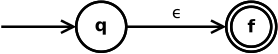
\includegraphics[scale=0.7]{empty.png}
\end{center}
- Kí tự $a \in A$:
\begin{center}
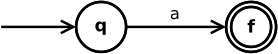
\includegraphics[scale=0.7]{symbol.png}
\end{center}
- Phép hợp $s+t$:
\begin{center}
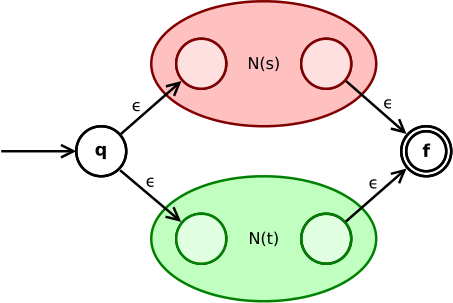
\includegraphics[scale=0.6]{union.png}
\end{center}
- Phép tích ghép $s.t$:
\begin{center}
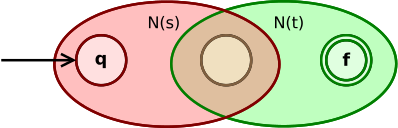
\includegraphics[scale=0.6]{concac.png}
\end{center}
- Phép $s^*$:
\begin{center}
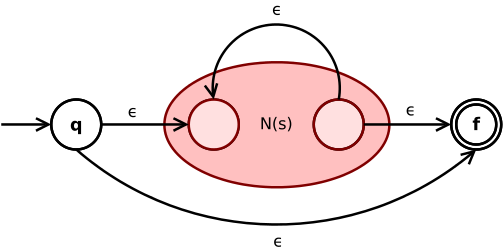
\includegraphics[scale=0.6]{star.png}
\end{center}

\begin{algorithm}[H]
\caption{Chuyển từ biểu thức chính quy sang NFA}
\begin{algorithmic} 
\STATE \textbf{Input} Biểu thức chính quy $s$
\STATE \textbf{Output} NFA $M = \{Q, A, \delta, q_0, F\}$
\STATE Duyệt biểu thức chính quy, thực hiện xây dựng NFA như mô tả bên trên.
\end{algorithmic}
\end{algorithm}
%----------------------------------------------------------------------------------
--------------------------------------------------------------------------------\\
\begin{algorithm}[H]
\caption{Chuyển từ biểu thức chính quy sang DFA}
\begin{algorithmic} 
\STATE \textbf{Input} Biểu thức chính quy $s$
\STATE \textbf{Output} DFA $M = \{Q, A, \delta, q_0, F\}$
\STATE Thực hiện chuyển biểu thức chính quy sang NFA.
\STATE Từ NFA trên ta tiếp tục thực hiện chuyển từ NFA sang DFA, tối tiểu hóa nếu cần.
\STATE Từ đó ta có được DFA ứng với biểu thức chính quy đã cho.
\end{algorithmic}
\end{algorithm}
%----------------------------------------------------------------------------------
--------------------------------------------------------------------------------\\
\begin{algorithm}[H]
\caption{Chuyển từ văn phạm tuyến tính trái sang văn phạm tuyến tính phải}
\begin{algorithmic} 
\STATE \textbf{Input} Văn phạm tuyến tính trái $G_T = \{V_T, V_N, S, P\}$
\STATE \textbf{Output} Văn phạm tuyến tính phải $G_P = \{V_T', V_N', S', P'\}$
\IF{tồn tại luật có dạng $S \rightarrow Sw$ với $w \in V_T*$}
\STATE Thêm vào $V_N$ $S_0$, thêm luật $S_0 \rightarrow S$ vào $P$, đặt $S = S_0$.
\ENDIF
\STATE Khởi tạo $V_T' = V_T, V_N' = V_N, P' = \emptyset, S' = S$
\FOR{\textbf{each} luật $p \in P$}
\IF{luật có dạng $S \rightarrow p$}
\STATE Thêm luật đó vào $P'$
\ELSIF{luật có dạng $A \rightarrow p$}
\STATE Thêm luật $S \rightarrow pA$ vào $P'$
\ELSIF{luật có dạng $B \rightarrow Ap$}
\STATE Thêm luật $A \rightarrow pB$ vào $P'$
\ELSIF{luật có dạng $S \rightarrow Ap$}
\STATE Thêm luật $A \rightarrow p$ vào $P'$
\ENDIF
\ENDFOR
\end{algorithmic}
\end{algorithm}

%----------------------------------------------------------------------------------
--------------------------------------------------------------------------------\\
\begin{algorithm}[H]
\caption{Chuyển từ văn phạm chính quy sang NFA}
\begin{algorithmic} 
\STATE \textbf{Input} Văn phạm chính quy $G = \{V_T, V_N, S, P\}$
\STATE \textbf{Output} NFA $M = \{Q, A, \delta, q_0, F\}$ tương ứng với văn phạm đã cho.
\IF{Văn phạm $G$ là tuyến tính trái}
\STATE Chuyển $G$ về dạng tuyến tính phải
\ENDIF
\STATE Khởi tạo $A = V_T$
\FOR{\textbf{each} $v \in V_N$}
\STATE Tạo trạng thái $q_{v}$ mới tương ứng.
\STATE Thêm $q_{v}$ vào $Q$.
\ENDFOR
\STATE Gán $q_0 = q_S$
\STATE Thêm trạng thái $q_\epsilon$ vào $Q$, đặt $F = \{q_\epsilon\}$
\FOR{\textbf{each} luật $p \in P$}
\STATE Với $p = A \rightarrow wB$ trong đó $A \in V_N, B \in V_N \cup \{\epsilon\}, w \in V_T^*, w = w_1.w_2...w_n$
\STATE Thêm các trạng thái $q_{pw_1}, q_{pw_2}, ..., q_{pw_{n-1}}$ vào $Q$.
\STATE Gán $\delta(q_{pw_i}, w_{i+1}) = q_{pw_{i+1}}$ với $i=1,...,n-2$.
\STATE Gán $\delta(q_A, w_1) = q_{pw_1}$, $\delta(q_{pw_{n-1}}, w_n) = q_B$.
\ENDFOR
\end{algorithmic}
\end{algorithm}

%----------------------------------------------------------------------------------
--------------------------------------------------------------------------------\\
\begin{algorithm}[H]
\caption{Chuyển từ NFA sang văn phạm tuyến tính phải}
\begin{algorithmic} 
\STATE \textbf{Input} NFA $M = \{Q, A, \delta, q_0, F\}$
\STATE \textbf{Output} Văn phạm tuyến tính phải $G = \{V_T, V_N, S, P\}$ tương ứng với NFA đã cho.
\STATE Khởi tạo $V_T = A, V_N = Q, S = q_0$
\FOR{\textbf{each} $q_i \in Q$}
\FOR{\textbf{each} $a \in A$}
\FOR{\textbf{each} $q_j \in \delta(q_i, a)$}
\STATE Thêm luật $q_i \rightarrow aq_j$ vào $P$
\ENDFOR
\ENDFOR
\ENDFOR
\FOR{\textbf{each} $q_i \in F$}
\STATE Thêm luật $q_i \rightarrow \epsilon$ vào $P$
\ENDFOR
\end{algorithmic}
\end{algorithm}

%----------------------------------------------------------------------------------
--------------------------------------------------------------------------------\\
\begin{algorithm}[H]
\caption{Chuyển từ văn phạm chính quy sang biểu thức chính quy}
\begin{algorithmic} 
\STATE \textbf{Input} Văn phạm chính quy $G = \{V_T, V_N, S, P\}$
\STATE \textbf{Output} Biểu thức chính quy ứng với văn phạm đã cho
\STATE Chuyển văn phạm chính quy về NFA
\STATE Từ NFA thực hiện chuyển về biểu thức chính quy.
\end{algorithmic}
\end{algorithm}

%----------------------------------------------------------------------------------
--------------------------------------------------------------------------------\\
\begin{algorithm}[H]
\caption{Chuyển từ biểu thức chính quy sang văn phạm chính quy}
\begin{algorithmic} 
\STATE \textbf{Input} Biểu thức chính quy $s$
\STATE \textbf{Output} Văn phạm chính quy $G = \{V_T, V_N, S, P\}$ ứng với biểu thức chính quy đã cho
\STATE Chuyển biểu thức chính quy về NFA
\STATE Từ NFA thực hiện chuyển về văn phạm tuyến tính phải. Đây cũng chính là văn phạm chính quy cần tìm.
\end{algorithmic}
\end{algorithm}

\chapter{Sơ lược về lý thuyết mã}
\section{Mã}
$A$ là bảng chữ. $X$ được gọi là mã nếu $\forall m,n$ và $x_1,x_2,...,x_n,y_1,y_2,...,y_m \in X$ thỏa mãn điều kiện:
\begin{center}
$x_1x_2...x_n=y_1y_2...y_m$
\end{center}
khi đó, $m=n$ và $x_i=y_i,i=\overline{1,n}$ \\
Hay nói cách khác, một tập $X$ là mã nếu tất cả các từ trong $X^+$ đều chỉ có một cách phân tích duy nhất thành các từ trong $X$.
Từ định nghĩa trên ta dễ thấy tập con của một mã cũng là một mã, và mã không thể chứa kí tự $\epsilon$
\subsection{Tính chất của mã}
Định nghĩa về mã còn có thể phát biểu bằng một cách khác như sau\\
\textbf{Bổ đề 1.1} Cho $X$ là tập con của $A^*$ là một mã, khi đó nếu một đồng cấu $\beta : B^* \rightarrow A^*$ chứa một song anh đi từ $B$ vào $X$ thì nó là đơn ánh. Ngược lại nếu tồn tại một đồng cấu đơn ánh $\beta : B^* \rightarrow A^*$ sao cho $X = \beta(B)$ thì $X$ là một mã. \\
Bổ đề 1.1 là lý do tại sao một tập $X$ được gọi là mã. Bản chất của việc mã hóa là tương ứng một kí tự $b \in B^*$ với một kí tự $a \in A^*$ theo một quy tắc mã hóa $\beta$ nào đó. Việc $\beta$ là đơn ánh đảm bảo rằng việc giải mã các xâu nhận được từ việc mã hóa là duy nhất.\\

\textbf{Hệ quả 1.2.} Cho $\alpha : A^* \rightarrow C^*$ là một đồng cấu và đơn ánh. Khi đó, nếu $X$ là một mã trên $A$ thì $\alpha (X)$ là một mã trên $C$. Ngược lại, ta cũng có, nếu $Y$ là một mã trên $C$, thì $\alpha^{-1}(Y)$ cũng là một mà trên $A$ \\

\textbf{Hệ quả 1.3.} Nếu $X \subset A^*$ là một mã, thì $X^n$ cũng là một mã trện $A \ \forall \ n > 0$
\subsection{Các loại mã đặc biệt}
Cho $X$ là một tập con của $A^*$. Khi đó, $X$ được gọi là tập prefix nếu không phần tử nào trong $X$ là prefix của phần tử khác trong $X$. Nếu ta xây dựng một quan hệ thứ tự prefix $x \leq x'$ nếu $x$ là prefix của $x'$, thi khi đó $X$ là một mã nếu mọi phần tử $ x, x'$ trong $X$ mà $x \leq x'$ thì $x = x'$. Hay nói cách khác, $X$ là một mã nếu hai phần tử phân biệt bất kì trong $X$ đều không thể so sánh được với nhau theo quan hệ thứ tự prefix. \\
Từ định nghĩa trên, ta dễ thấy rằng nếu một tập prefix chứa kí tự $\epsilon $ thì tập đó chỉ chứa duy nhất một kí tự là $\epsilon$.\\
Tập suffice được định nghĩa bằng một cách tương tự: Tập suffix là tập mọi phần tử đều không là suffix của các phần tử khác trong nó. Một tập là biprefix khi nó vừa là tập prefix, vừa là tập suffix. \\
\textbf{Bổ đề 1.4} Mọi tập prefix (suffix, biprefix) khác $\{ \epsilon \} $ đều là một mã.
\textbf{Chứng minh.} Giả sử rằng $X$ không phải là mã, khi đó tồn tại ít nhất một xâu $w$ có hai cách phân tích khác nhau. Gọi xâu có độ dài ngắn nhất như vậy là $w$
$$w = x_1x_2...x_n = x_1'x_2'...x_m'$$
Vì $x_1, x_1'$ khác kí tự rỗng, và $w$ là xâu có độ dài ngắn nhất nên $x_1 \neq x_1'$. Khi đó $x_1 < x_1'$ hoặc $x_1' < x_1$, mâu thuẫn với giả thiết của tập prefix. Vậy tập prefix là mã. Ta cũng có thể có chứng minh tương tự đối với tập suffix.

\subsection{Mã tối đại}
Mã $X$ được gọi là tối đại (theo nghĩa bao hàm) trên $A$ nếu $X$ không là con thực sự trong một mã nào khác trên $A$.\\
Chú ý rằng tính tối đại của một mã phụ thuộc vào bảng chữ cái mà nó được xây dựng lên. Nếu $X \subset A^*$ là một mã tối đại trên $A$ và $A$ là tập con thực sự của $B$ thì khi đó $X$ không đảm bảo là mã tối đại trên $B$.\\
\textbf{Bổ đề 1.5} Cho $A$ là một bảng chữ cái. Khi đó mọi ví nhóm con $M$ thuộc $A^*$ đều có duy nhất một tập sinh cực tiểu $X = (M-1) - (M-1)^2$\\
\textbf{Bổ đề 1.6} Nếu $M$ là một vị nhóm tự do con của $A^*$, khi đó tập sinh cực tiểu của $M$ là một mã. Ngược lại, nếu $X \subset A^*$ là một mã, thì vị nhóm con $X^*$ là vị nhóm tự do và $X$ là tập sinh cực tiểu của nó.\\
\textbf{Bổ đề 1.7} Nếu $M$ là vị nhóm con tự do tối đại của $A^*$ thì cơ sở $X$ của nó là mã tối đại.

\section{Tiêu chuẩn kiểm định mã}
Bài toán kiểm định một tập cho trước là một mã hay không là bài toán khó. Trong phần này, thuật toán được miêu tả không sử dụng các tính chất đặc biệt của mã mà chỉ sử dụng các phép tính toán hợp lý để kiểm định mã và thuật toán chỉ có thể thực hiện được với mã hữu hạn. \\
Thuật toán được trình bày dưới đây tính tất cả các phần dư của mọi cách thử phân tích xâu thành hai cách khác nhau. Thuật toán phát hiện được một xâu tồn tại nhiều hơn 2 cách phân tích khác nhau khi phần dư chứa kí tự rỗng $\epsilon$\\
Một cách cự thể, các phần dư được thực hiện lần lượt như sau. Gọi $X$ là một tập con của $A^*$, và
$$U_1 = X^{-1} X - \epsilon$$
$$U_{n+1} = X^{-1} U_n \cup U_n^{-1} X$$
Trong đó $N^{-1}D = \{y | xy \in D \ và \ x \in N  \}$ \\
Khi đó ta có kết quả sau: \\
\textbf{Định lý 2.1} Tập $X \subset A^*$ là một mã khi và chỉ khi các tập $U_n$ không chứa kí tự rỗng (với mọi $n$). \\
\textbf{Bổ đề 2.2} Nếu $X$ là tập một tập hữu hạn thì tập các $U_n$ là một tập hữu hạn \\
Chú ý rằng ta dễ có kết quả của bổ đề 2.2 vì $U_n$ chỉ gồm suffix của những xâu trong $X$

Từ hai kết quả trên, ta có thể miêu tả thuật toán kiểm định mã cho một tập hữu hạn $X$ như sau
Bài toán:
\begin{itemize}
\item Input: Một tập $X$ gồm hữu hạn các xâu thuộc $A^+$
\item Output: $X$ có phải phải là mã hay không ?
\end{itemize}

\begin{enumerate}
\item Tính $S_1 = X^{-1}X \setminus \{ \epsilon \}$
\item Thực hiện vòng lặp tính và lưu lại giá trị của $U_{i+1}$ theo công thức
$$U_{n+1} = X^{-1} U_n \cup U_n^{-1} \ với \ i \geq 1$$
\item Nếu trong quá trình tính toán, tại một giá trị $i$ nào đó mà $U_n$ chứa kí tự rỗng thì dừng thuật toán và kết luận $X$ không phải là mã.
\item Nếu trong quá trình tính toán, tìm được $U_j$ mà $U_{j} = U_i$ với $i < j$ thì dừng thuật toán và kết luận $X$ là mã
\end{enumerate}

Đính lý 2.1 và bổ đề 2.2 giúp khẳng định rằng thuật toán trên sẽ dừng sau một số hữu hạn bước tính toán.

\chapter{Ứng dụng của lý thuyết mã}
\section{Single-Error Correcting Codes}
\section{Lossless Data Compression}




\chapter{Kết luận}
Bài báo cáo đã hoàn thành trình bày kiến thức cơ sở và những tính chất quan trọng của ngôn ngữ chính quy. Giải quyết được khá nhiều bài toán liên quan đến việc biểu diễn một ngôn ngữ chính quy. Tuy nhiên vẫn còn nhiều vấn đề chưa được giải quyết như việc rút gọn biểu thức thức chính quy, hay một số thuật toán được miêu tả trong chương 4 vẫn có độ phức tạp mũ. Mặc dù thuật toán Sardinas-Partison được trình bày trong phần kiểm định mã có thể mở rộng cho trường hợp tập $X$ là tập vô hạn có thể nhận biết được (recognizable set), chương 5 đã trình bày sơ lược về lý thuyết mã khá hoàn chỉnh. Bên cạnh các vấn đề về lý thuyết, bài báo cáo cũng trình bày về mã sửa sai - một ứng dụng khá quan trọng lý thuyết mã hóa.
Lời cuối cùng, nhóm chúng em xin cảm ơn cô Ngô Thị Hiền đã giúp đỡ và hướng dẫn nhóm chúng em hoàn thiện bài báo này.
\newpage
{\huge \textbf{Tài liệu tham khảo}} \\
[1] Introduction to Automata Theory, Languages, and Computation, \textit{John E. Hopcroft, Rajeev Motwani, Jeffray D.Ullman}
[2] A Necessary and Sufficient Pumping Lemma for Regular Languages, \textit{Jeffrey Jaffe, 1978}
[3]
\end{document}
